\documentclass[15pt,aspectratio=169]{beamer}

\usepackage[pdf]{graphviz}

\usetheme{metropolis}
\usepackage{appendixnumberbeamer}

\usepackage{booktabs}
\usepackage[scale=2]{ccicons}

\usepackage{pgfplots}
\usepgfplotslibrary{dateplot}

\usepackage{xspace}

\usepackage{labslide}

\addbibresource{references.bib}

\title{Title}
\subtitle{Subtitle}
\date{\today}
\author{Jeff Dean}
\institute{B4, Snivy Lab.}
\titlegraphic{\hfill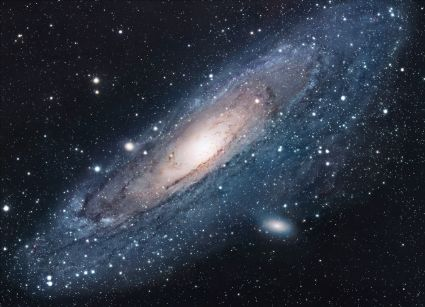
\includegraphics[height=1.5cm]{universe.jpg}}

\begin{document}

\maketitle

\begin{frame}{Table of contents}
    \tableofcontents[hideallsubsections]
\end{frame}

\section{Introduction}

\begin{frame}{Introduction}

Objective\footfullcite{adams1995hitchhiker}

\begin{itemize}
    \item Foo
    \item Bar
    \item Buzz
\end{itemize}
    
\end{frame}

\begin{frame}{Alice and Bob}
    In a context of cryptography, these names are used to represent people.
    
    \begin{table}[]
        \centering
        \caption{Person names}
        \begin{tabular}{c|c}
             Name & Description \\ \hline
             Alice & Sender \\
             Bob & Receiver  \\
             Eve & Eavesdropper \\
             Mallory & Malicious attacker \\
             Trent & Trusted third party \\
             Victor & Verifier
        \end{tabular}
        \label{tab:my_label}
    \end{table}
\end{frame}

\begin{frame}{Digraph Example}
    \digraph[scale=0.5]{hoge}{a->b->c;}
\end{frame}

\section{Related Work}

\section{Proposed Method}

\section{Experiment}

\section{Conclusion}

\begin{frame}{Summary}

  Get the source of this theme and the demo presentation from

  \begin{center}\url{github.com/matze/mtheme}\end{center}

  The theme \emph{itself} is licensed under a
  \href{http://creativecommons.org/licenses/by-sa/4.0/}{Creative Commons
  Attribution-ShareAlike 4.0 International License}.

  \begin{center}\ccbysa\end{center}

\end{frame}

\begin{frame}[allowframebreaks]{References}
\printbibliography[heading=none]
\end{frame}

\begin{frame}[standout]
  Questions?
\end{frame}

\appendix

\begin{frame}[fragile]{Backup slides}
  Sometimes, it is useful to add slides at the end of your presentation to
  refer to during audience questions.

  The best way to do this is to include the \verb|appendixnumberbeamer|
  package in your preamble and call \verb|\appendix| before your backup slides.

  \themename will automatically turn off slide numbering and progress bars for
  slides in the appendix.
\end{frame}

\end{document}